\input ../SlidePreamble
\input ../preamble


\begin{document}

{\Huge

  \centerline{\bf TTIC 31230, Fundamentals of Deep Learning}
  \bigskip
  \centerline{David McAllester, Winter 2019}
  \vfill
  \centerline{Entropy and Compressibility}
  \vfill
  \centerline{Rate-Distortion Autoencoders (RDAs)}
  \vfill
  \centerline{Noisy Channel RDAs}
  \vfill
  \centerline{Gaussian Variational Autoencoders (Gaussian VAEs)}

\slide{Issue I: Measuring Cross Entropy}

We typically cannot measure cross-entropy for a graphical model.

\vfill
But we can measure cross-entropy of a compression model.

\vfill
We write $\tilde{z}(y)$ for a lossless compression of $y$ and write $|\tilde{z}_\Phi(y)|$ for the bit length of the compression.

\vfill
{\color{red}
\begin{eqnarray*}
\Phi^* & = & \argmin_\Phi \;E_{y \sim \pop} \;-\ln P_\Phi(y) \\
\\
\Phi^* & = & \argmin_\Phi \;E_{y \sim \pop} \;|\tilde{z}_\Phi(y)|\;\;\;\mbox{such that $\forall y\;\;\;y = \tilde{y}_\Phi(\tilde{z}_\Phi(y))$}
\end{eqnarray*}
}

\slide{Issue II: Avoiding Differential Entropy}

For reasons discussed below, we would like to avoid differential entropy.

\vfill
To avoid differential entropy we use a rate-distortion objective.

\vfill
{\color{red} \huge
\begin{eqnarray*}
\Phi^* & = & \argmin_\Phi \;E_{y \sim \pop} \;-\ln P_\Phi(y)\;\;\;\mbox{$y$ discrete} \\
\\
\Phi^* & = & \argmin_\Phi \;E_{y \sim \pop} \;-\ln P_\Phi(\tilde{y}_\Phi(y)) + \lambda \mathrm{Dist}(y,\tilde{y}_\Phi(y))
\left\{\begin{array}{l}\mbox{$y$ continuous} \\ \mbox{$\tilde{y}$ discrete}\end{array}\right.
\end{eqnarray*}
}

\slide{Lossy Compression}

Lossy compression combines compression for measuring cross-entropy with distortion for avoiding differential entropy.

\vfill
{\color{red}
\begin{eqnarray*}
\Phi^* & = & \argmin_\Phi \;E_{y \sim \pop} \;-\ln P_\Phi(y) \\
\\
\Phi^* & = & \argmin_\Phi \;E_{y \sim \pop} \;|\tilde{z}_\Phi(y)| + \lambda \mathrm{Dist}(y,\tilde{y}_\Phi(\tilde{z}_\Phi(y)))
\end{eqnarray*}
}



\slide{Entropy and Compression}

For a distribution $P(y)$ on a discrete set ${\cal Y}$, the entropy $H(P)$, when measured using $\log_2$ rather than $\ln$, gives the number of bits needed
on average, when drawing from $P$, to represent the elements of ${\cal Y}$.

\vfill
The cross-entropy $H(P,Q)$ give the number of bits used to code for items drawn from $P$ but using the code defined by $Q$.

\vfill
Cross-entropy gives the ``data rate'' when transmitting codes for items drawn from $P$ but using the code defined by $Q$.

\slide{Entropy and Compressibility}

Let $S$ be a finite set.

\vfill
Let $z$ be a compression (or coding) function  assigning a bit string $z(y)$ to each $y \in S$.

\vfill
The compression function $z$ is called {\em prefix-free} if for $y' \not = y$ we have that $z(y')$ is not a prefix of $z(y)$.

\slide{Prefix-Free Codes as Probabilities}

A prefix-free code defines a binary branching tree --- branch on the first code bit, then the second, and so on.

\vfill
For a prefix-free code, only the leaves of this tree can be labeled with the elements of $S$.

\vfill
The code defines a probability distribution on $S$ by randomly selecting branches.

\vfill
We have $P_z(y) = 2^{-|z(y)|}$.

\slide{Bits vs. Nats}

We have that $|z(y)|$ is a number of bits.

\vfill
We can define entropy in units of bits by

\vfill
$$H_2(y) = E_y\; - \log_2 P(y) = H(y)/(\ln \;2)$$

\vfill
If $y$ is uniformly distributed over 8 values then $H_2(y)$ is 3 bits.

\vfill
We have that $H_2(y)$ is a number of bits while $H(y)$ is a number of ``nats''.

\slide{The Source Coding (compression) Theorem}

(1) There exists a prefix-free code $z$ such that
$$|z(y)| <= (- \log_2 \mathrm{Pop}(y)) + 1$$
and hence
$$E_{y\sim \mathrm{Pop}} |z(y)| \leq H_2(\mathrm{Pop}) +1$$

\vfill
(2) For any prefix-free code $z$

$$E_{y \sim \mathrm{Pop}}\;|z(y)| \geq H_2(\mathrm{Pop})$$

\slide{Code Construction}

\vfill
We construct a code by iterating over $y \in S$ in order of decreasing probability (most likely first).

\vfill
For each $y$ select a code word $z(y)$ (a tree leaf) with length (depth)

\vfill
$$|z(y)| = \lceil - \log_2 \mathrm{Pop}(y)\rceil$$

\vfill
and where $z(y)$ is not an extension of (under) any previously selected code word.

\slide{Code Existence Proof}

At any point before coding all elements of $S$ we have
$$\sum_{y \in \mathrm{Defined}} 2^{-|z(y)|} \leq \sum_{y \in \mathrm{Defined}} \mathrm{Pop}(y) < 1$$

\vfill
Therefore there exists an infinite descent into the tree that misses all previous code words.

\vfill
Hence there exists a code word $z(x)$ not under any previous code word with
$|z(x)| = \lceil - \log_2 \mathrm{Pop}(y)\rceil$.

\vfill
Furthermore $z(x)$ is at least as long as all previous code words and hence $z(x)$ is not a prefix of any previously selected code word.

\slide{No Better Code Exists}

Let $z$ be an arbirtary coding.

\begin{eqnarray*}
E_y\;|z(y)| & = & E_y\; -\log_2 P_z(y) \\
\\
 & = & H_2(\mathrm{Pop},P_z) \\
 \\
 &= & H_2(\mathrm{Pop}) + KL_2(\mathrm{Pop},P_z) \\
 \\
 &\geq & H_2(\mathrm{Pop})
\end{eqnarray*}
 
\slide{Huffman Coding}

Maintain a list of trees $T_1,\;\dots,\;T_N$.

\vfill
Inititally each tree is just one root node labeled with an element of $S$.

\vfill
Each tree $T_i$ has a weight equal to the sum of the probabilities of the nodes on the leaves of that tree.

\vfill
Repeatedly merge the two trees of lowest weight into a single tree until all trees are merged.

\slide{Optimality of Huffman Coding}

{\bf Theorem}: The Huffman code $T$ for $\mathrm{Pop}$ is optimal --- for any other tree $T'$ we have $H(\mathrm{Pop},T) \leq H(\mathrm{Pop},T')$.

\vfill
{\bf Proof}: The algorithm maintains the invariant that there exists an optimal tree including
all the subtrees on the list.

\vfill
To prove that a merge operation maintains this invariant we consider any tree containing the given subtrees.

\vfill
Consider the two subtrees $T_i$ and $T_j$ of minimal weight.  Without loss of generality we can assume that $T_i$ is at least as deep as $T_j$.

\vfill
Lowering $T_j$ to be the sibling of $T_i$ while raising the old sibling of $T_i$ to $T_j$'s original position
brings $T_i$ and $T_j$ together and can only improve the average depth.

\slide{Differential Entropy}

Consider a continuous density $p(x)$.  For example

\vfill
$$p(x) = \frac{1}{\sqrt{2\pi}\; \sigma}\; e^{\frac{-x^2}{2\sigma^2}}$$

\vfill
Differential entropy is often defined as

\vfill
$$H(p) \doteq \int \left(\ln \frac{1}{p(x)}\right) p(x) dx$$


\slide{Differential Entropy Depends on the Choice of Units}

\begin{eqnarray*}
  H({\cal N}(0,\sigma)) & = &  + \int \left( \ln(\sqrt{2\pi} \sigma) + \frac{x^2}{2\sigma^2}\right) p(x) dx \\
  \\
  & = & \ln(\sigma) + \ln(\sqrt{2\pi}) + \frac{1}{2}
\end{eqnarray*}

\vfill
But if we take $y \doteq x/2$ we get $H(y) = H(x) - \ln 2$.

\vfill
Also for $\sigma << 1$, we get $H(p) < 0$

\vfill
Hence differential entropy then depends on the choice of units --- a distributions on lengths will have a different entropy
when measuring in inches than when measuring in feet.

\slide{More Problems with Differential Entropy}

There are also other problems with continuous entropy and cross-entropy.

\vfill
\begin{itemize}
\item Finite continuous entropy violates the source coding theorem --- it takes an infinite number of bits to code a real number.

\vfill
\item Finite continuous entropy violates the data processing inequality that $H(f(x)) \leq H(x)$.  For a continuous random variable $x$ under finite continuous entropy we can have $H(f(x)) > H(x)$.
\end{itemize}

\vfill
For these reasons it seems advisable to avoide differential entropy and differential cross entropy.

\slide{Differential KL-divergence is Independent of Units}

$$KL(p,q) = \int \left( \ln \frac{p(x)}{q(x)}\right) p(x) dx$$

\vfill
This integral can be computed by dividing the real numbers into bins and computing the $KL$ divergence between the distributions on bins.

\vfill
The KL divergence between the bin distribution often approaches a finite limit as the bin size goes to zero.


\slide{Rate-Distortion Autoencoders}

Given a continuous signal $y$ we can compress it into a (discrete) bit string $\tilde{z}_\Phi(y)$.

\vfill
We let $\tilde{y}_\Phi(\tilde{z}_\Phi(y))$ be the decompression of $\tilde{z}_\Phi(y)$.

\vfill
We can then define a rate-distortion loss.

{\color{red} $${\cal L}(\Phi) = E_{y \sim \mathrm{Pop}}\;|\tilde{z}_\Phi(y)| + \lambda \mathrm{Dist}(y,\tilde{y}_\Phi(\tilde{z}_\Phi(y)))$$}

\slide{The Rate-Distortion Tradeoff}

{\color{red} $${\cal L}(\Phi) = E_{y \sim \mathrm{Pop}}\;|\tilde{z}_\Phi(y)| + \lambda \mathrm{Dist}(y,\tilde{y}(\tilde{z}(y)))$$}

\vfill
The first term is as a rate measured in in bits per sample.

\vfill
The meta-parameter $\lambda$ has units of inverse distortion and controls the trade off between rate and distortion.

\slide{Common Distortion Functions}

$$\Phi^* = \argmin_\Phi\;E_{y \sim \mathrm{Pop}}\;|\tilde{z}_\Phi(y)| + \lambda \mathrm{Dist}(y,\tilde{y}_\Phi(y))$$

\vfill
It is common to take

$$\mathrm{Dist}(y,\tilde{y}) = ||y-\tilde{y}||^2 \hspace{4em}(L_2)$$

\vfill
or

$$\mathrm{Dist}(y,\tilde{y}) = ||y-\tilde{y}||_1 \hspace{4em} (L_1)$$

\slide{A Case Study in Image Compression}

{\bf End-to-End Optimized Image Compression, Balle, Laparra, Simoncelli, ICLR 2017.}


\vfill
$${\color{red}y \hspace{5em}  \tilde{z}_\Psi(y) \hspace{4em} \tilde{z} \hspace{6em} \tilde{y}_\Phi(\tilde{z}) \hspace{4em}||y - \tilde{y}||^2}$$
\centerline{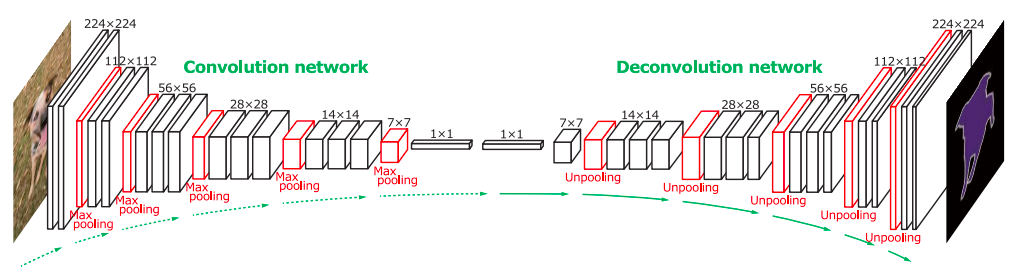
\includegraphics[width=9in]{../images/Deconv}}

\anaslide{JPEG at 4283 bytes or .121 bits per pixel}

\bigskip
\centerline{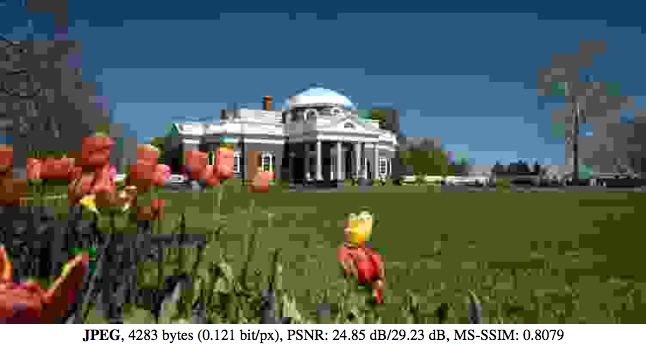
\includegraphics[height=5in]{../images/RateDist2}}

\anaslide{JPEG 2000 at 4004 bytes or .113 bits per pixel}

\bigskip
\centerline{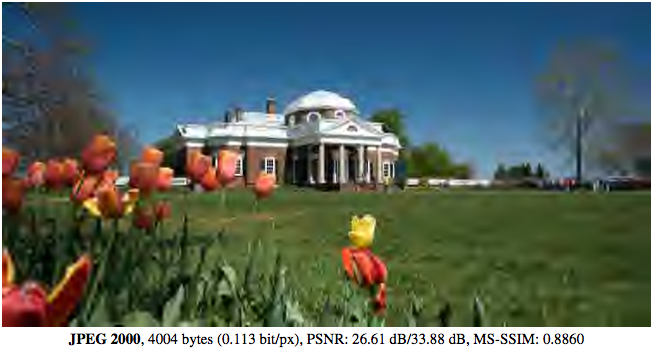
\includegraphics[height= 5in]{../images/RateDist3}}

\anaslide{Deep Autoencoder at 3986 bytes or .113 bits per pixel}

\bigskip
\centerline{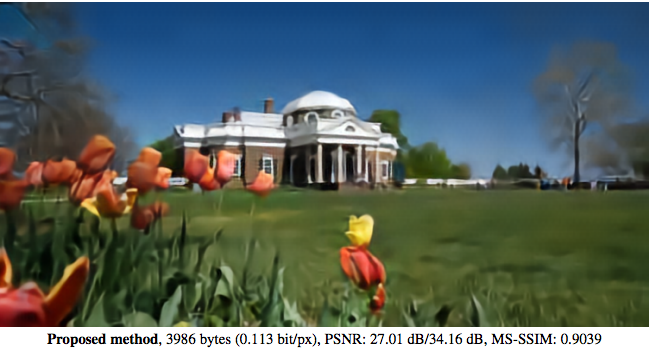
\includegraphics[height = 5in]{../images/RateDist4}}

\slide{A CNN Encoder}

A three layer CNN is used as an encoder.

\vfill
We let $z_\Phi(y)$ be the final layer of this CNN.

\vfill
Each continuous value in the final layer $z_\Phi(y)$ is then rounded to a (small) integer giving a discrete encoding $\tilde{z}(y)$.

\slide{Rate-Distortion Autoencoders}

$$\Phi^* = \argmin_\Phi \;E_{y \sim \pop}\;|\tilde{z}_\Phi(y)| + \lambda \mathrm{Dist}(y,y_\Phi(\tilde{z}_\Phi(y)))$$

\vfill
Oops: Because of rounding, $\tilde{z}_\Phi(y)$ is discrete and the gradients are zero.

\slide{Rate-Distortion Autoencoders}

\begin{eqnarray*}
\Phi^* & & = \argmin_\Phi {\cal L}_{\mathrm{rate}}(\Phi) + \lambda {\cal L}_{\mathrm{dist}} (\Phi) \\
\\
{\cal L}_{\mathrm{rate}}(\Phi) & = & E_{y \sim \pop}\;|\tilde{z}_\Phi(y)| \\
\\
{\cal L}_{\mathrm{dist}}(\Phi) & = & E_{y \sim \mathrm{Pop}} \;\mathrm{Dist}(y,y_\Phi(\tilde{z}_\Phi(y)))
\end{eqnarray*}

\vfill
We will consider differentiable approximations to both ${\cal L}_{\mathrm{rate}}$ and ${\cal L}_{\mathrm{dist}}$.

\slide{A Differentiable Approximation of ${\cal L}_{\mathrm{rate}}$}

\begin{eqnarray*}
{\cal L}_{\mathrm{rate}}(\Phi) & = & E_{y \sim \pop}\;|\tilde{z}_\Phi(y)| 
\end{eqnarray*}

\vfill
Recall that {\color{red} $\tilde{z}_\Phi(y)$} is a rounding of a continuous encoding {\color{red} $z_\Phi(y)$}.


\vfill
We can make the cross-entropy loss differentiable by approximating discrete entropy with differential entropy.

\vfill
$$|{\color{red} \tilde{z}_\Phi(y)}| \approx - \ln p_\Psi({\color{red} z_\Phi(y)})\;\;\;\;\;\;\;p_\Psi(z) \approx \sum_i \log_2 z_i$$


\slide{Differential Entropy vs. Discrete Entropy}

\bigskip
\centerline{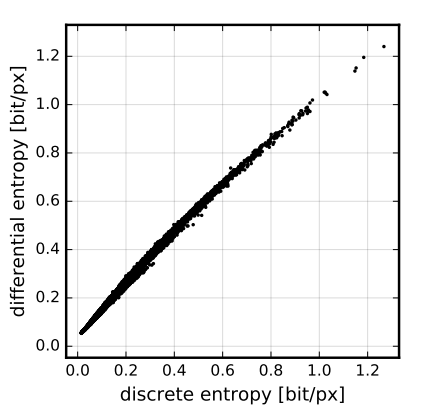
\includegraphics[height=5in]{../images/RateDist6}}

\slide{A Differentiable Approximation of ${\cal L}_{\mathrm{dist}}$}

We can make the the distortion loss differentiable by modeling rounding as the addition of noise.

\begin{eqnarray*}
{\cal L}_{\mathrm{dist}}(\Phi) & = & E_{y \sim \mathrm{Pop}} \;\mathrm{Dist}(y,y_\Phi(\tilde{z}_\Phi(y))) \\
\\
& \approx & E_{y,\epsilon} \;\mathrm{Dist}(y,\;y_\Phi(z_\Phi(y) + \epsilon))
\end{eqnarray*}

\vfill
Here $\epsilon$ is a noise vector each component of which is drawn uniformly from $(-1/2,1/2)$.

\slide{Noise vs. Rounding}

\centerline{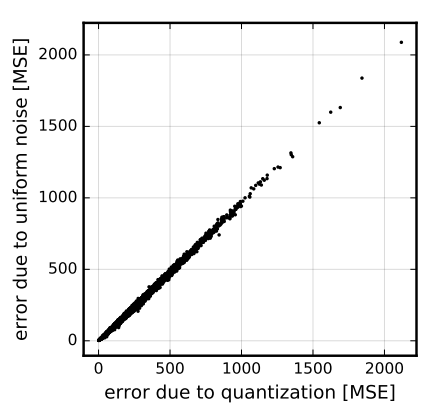
\includegraphics[height=5in]{../images/RateDist5}}

\slide{Details}

\vfill
The first layer is computed stride 4.

\vfill
The next two layers are computed stride 2.

\vfill
Final image dimension is reduced by a factor of 16 with 192 channels per pixel (192 channels is for color images).

\vfill
$$192 < 16 \times 16 \times 3 = 768$$

\vfill


\slide{Increasing Spatial Dimension in Decoding}

\centerline{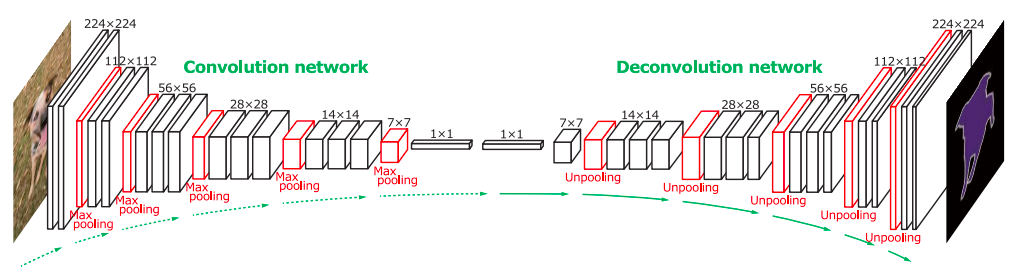
\includegraphics[width=9in]{../images/Deconv}}
\centerline{[Hyeonwoo Noh et al.]}

\vfill
In the ICLR 17 paper the deconvolution network has the shape as the input CNN but with independent parameters.

\slide{Increasing Spatial Dimension in Decoding}

Consider a stride 2 convolution
\begin{eqnarray*}
  L_{\ell+1}[x,y,j] & = & \sigma\left(\sum_{\Delta x,\Delta y,i}   W[\Delta x, \Delta y, i,j] L_\ell[2x + \Delta x, 2y + \Delta y, i]\right)
\end{eqnarray*}

\vfill
For deconvolution we use stride 1 with 4 times the features.
\begin{eqnarray*}
  L'_\ell[x,y,i] & = & \sigma\left(\sum_{\Delta x,\Delta y,j}   W[\Delta x, \Delta y, j,i] L'_{\ell+1}[x + \Delta x, y + \Delta y, j]\right)
\end{eqnarray*}

\vfill
The channels at each $L'_\ell[x,y]$ are divided among four higher resolution pixels.

\vfill
This is done by a simple reshaping of $L'_\ell[x,y,i]$.

\slide{Noisy-Channel RDAs (TZ)}

Consider the differentiable loss used in training.
{\color{red} $$\Phi^* = \argmin_\Phi \;E_{y \sim \pop}\;- \ln p(z_\Phi(y)) + \lambda E_\epsilon\; \mathrm{Dist}(y,y_\Phi(z_\Phi(y) + \epsilon))$$}

Intuitively, {\color{red} $- \ln p(z_\Phi(y))$} is a proxy for the number of bits used in the (intuitively rounded) encoding {\color{red} $z_\Phi(y) + \epsilon$}.

\vfill
By the channel capcacity theorem the number of bits that {\color{red} $z_\Phi(y) + \epsilon$} can carry about {\color{red} $y$}
is the mutual information between $y$ and $z_\Phi(y) + \epsilon$.

{\color{red} $$I(y,z_\Phi(y)+\epsilon)$$}

\slide{Noisy-Channel RDAs (TZ)}

We now consider {\color{red} $p_\Phi(z|y)$} as a generalization of {\color{red} $z_\Phi(y) + \epsilon$}.

\vfill
The channel capacity theorem motivates

\vfill
{\huge
\begin{eqnarray*}
{\color{red} \Phi^*} & = & {\color{red} \argmin_\Phi \left(\;I(y,z) + \;\lambda E_{y \sim \pop,z \sim p_\Phi(z|y)}\;\mathrm{Dist}(y,y_\Phi(z))\;\right)} \\
\\
& = & {\color{red} \argmin_\Phi  E_{y \sim \pop}\;\left(\;KL(p_\Phi(z|y),p_\Phi(z)) + \lambda E_{z \sim p_\Phi(z|y)}\; \mathrm{Dist}(y,y_\Phi(z))\;\right)} \\
\end{eqnarray*}
}

\slide{A Variational Upper Bound}

Unfortunately we cannot compute {\color{red} $p_\Phi(z) = E_{y \sim \pop}\;p_\Phi(z|y)$}.

\vfill
We now replace {\color{red} $p_\Phi(z)$} by a friendly (variational) model {\color{red} $p_\Psi(z)$}.

\begin{eqnarray*}
I_\Phi(y,z) & = & E_{y \sim \pop}\; KL(p_\Phi(z|y),p_\Phi(z)) \\
\\
& = & E_{y,z\sim P_\Phi(z|y)}\; \ln \frac{p_\Phi(z|y)}{{\color{red} p_\Psi(z)}} + \ln \frac{{\color{red} p_\Psi(z)}}{p_\Phi(z)} \\
\\
& = & E_y\;KL(p_\Phi(z|y),p_\Psi(z)) - KL(p_\Phi(z),p_\Psi(z)) \\
\\
& \leq & E_y\;KL(p_\Phi(z|y),p_\Psi(z))
\end{eqnarray*}

\slide{The Noisy-Channel RDA}

{\huge {\color{red} $$\Phi^*,\Psi^* = \argmin_{\Phi,\Psi}\;E_y \;KL(p_\Phi(z|y),P_\Psi(z)) \;+\; \lambda \; E_{z\sim p_\Phi(z|y)}\;\mathrm{Dist}(y,\;y_\Phi(z))$$}}

\vfill
Here $\gamma$ has the same units as distortion and controls the trade-off between rate and distortion.

\slide{Summary: Rate-Distortion}


Rate-Distortion: $y$, continuous, $\tilde{z}$ a bit string,

{\color{red}
\begin{eqnarray*}
\Phi^* &  = &  \argmin_\Phi E_y \;|\tilde{z}_\Phi(y)| + \lambda \mathrm{Dist}(y,y_\Phi(\tilde{z}_\Phi(y)))
\end{eqnarray*}
}

\vfill
Noisy Channel: {\color{red} $\tilde{z} = z_\Phi(y) + \sigma_\Phi(y) \odot \epsilon$,\hspace{2em} $\epsilon \sim {\cal N}(0,I)$}

{\color{red}
\begin{eqnarray*}
\Phi^* & = & \argmin_\Phi E_y\; \;KL(p_\Phi(\tilde{z}|y),{\cal N}(0,I)) + E_{\tilde{z}\sim p_\Phi(\tilde{z}|y)}\;\lambda \mathrm{Dist}(y,y_\Phi(\tilde{z}))
\end{eqnarray*}
}

\slide{END}

}
\end{document}

